\chapter{Fundamentos Geofísicos}

\section{Campo potencial gravitatorio}

Según la Ley de Gravitación Universal de Newton, una masa puntual $m_p$ situada
en la posición $\mathbf{p}$ siente una fuerza gravitatoria $\mathbf{F}$ debido
a la presencia de otra masa $m$ situada en la posición $\mathbf{q}$. Esta
fuerza puede expresarse como:

\begin{equation}
    \mathbf{F} = - G \frac{m_p m}{r^2} \mathbf{\hat{r}},
\end{equation}

\noindent donde $\mathbf{r} = \mathbf{p} - \mathbf{q}$ es el vector que va
desde la posición $\mathbf{q}$ a $\mathbf{p}$, y $G = 6.67430 \times
10^{-11} \text{m}^3 \text{kg}^{-1} \text{s}^{-2}$ es la constante de
gravitación universal (Fig.~\ref{fig:potencial-gravitatorio}a).
De esto se deduce que la masa $m_p$ siente una aceleración gravitatoria

\begin{equation}
    \mathbf{g} = - \frac{G m}{r^2} \mathbf{\hat{r}}.
    \label{eq:aceleracion-newton}
\end{equation}

Si consideramos que la partícula $m_p$ es una \emph{partícula de prueba},
podemos reescribir la ecuación \ref{eq:aceleracion-newton}, pero ahora
resignificándola como la aceleración gravitatoria que sentiría cualquier
partícula localizada en un punto $\mathbf{p}$ debido a la presencia de la
partícula $m$:

\begin{equation}
    \mathbf{g}(\mathbf{p}) = - \frac{G m}{r^2} \mathbf{\hat{r}}.
\end{equation}

Se puede demostrar que la atracción gravitatoria $\mathbf{g}$ define un campo
irrotacional, es decir

\begin{equation}
    \nabla \times \mathbf{g} = 0,
\end{equation}

\noindent por ende es posible definir un potencial escalar $V$ al que
denominaremos \emph{potencial gravitatorio}:

\begin{equation}
    \mathbf{g}(\mathbf{p}) = + \nabla V(\mathbf{p}),
    \label{eq:potencial-gravitatorio-definicion}
\end{equation}

\noindent donde

\begin{equation}
    V(\mathbf{p}) = G \frac{m}{r}.
\end{equation}

\noindent Vale la pena notar que en la ecuación
\ref{eq:potencial-gravitatorio-definicion} se ha utilizado la convención de
signo positivo para definir el potencial $V$, mayormente utilizada en la
bibliografía geofísica.

\begin{figure}
    \centering
    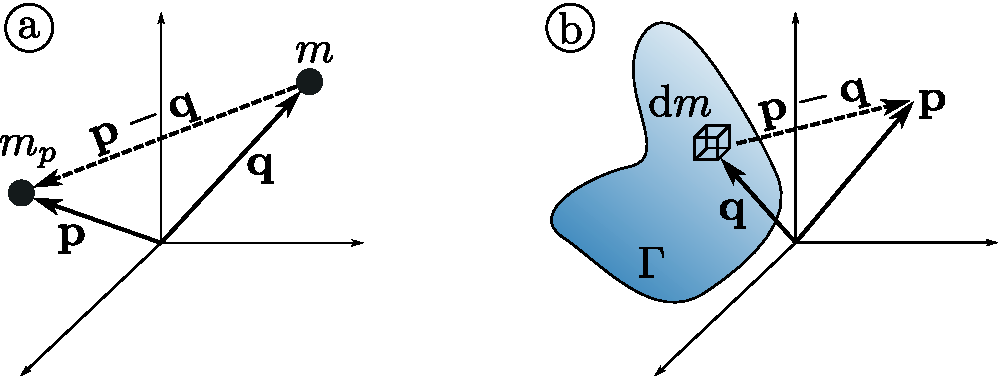
\includegraphics[width=\linewidth]{figs/gravity-potentials.pdf}
    \caption{
        (a)~Masas puntuales $m_p$ y $m$ localizadas en $\mathbf{p}$
        y $\mathbf{q}$, respectivamente. El vector $\mathbf{r}$ se define como
        $\mathbf{p} - \mathbf{q}$.
        (b)~Distribución de masa $\Gamma$, diferencial de masa $\text{d}m$
        ubicado en el punto $\mathbf{q}$.
    }
    \label{fig:potencial-gravitatorio}
\end{figure}

\subsection{Potencial gravitatorio producido por una distribución de masa}

Partiendo de que un diferencial de masa $\text{d}m$ ubicado en $\mathbf{q}$
genera un potencial gravitatorio $\text{d}V$ en cualquier punto $\mathbf{p}$
(Fig.~\ref{fig:potencial-gravitatorio}b):

\begin{equation}
    \text{d}V(\mathbf{p}) = \frac{G}{|\mathbf{p} - \mathbf{q}|} \text{d}m,
\end{equation}

\noindent el potencial gravitatorio generado por una distribución de masa
$\Gamma$ puede calcularse integrando los diferenciales de masa que lo componen:

\begin{equation}
    V(\mathbf{p}) = G \int\limits_\Gamma \frac{\text{d}m}{|\mathbf{p} - \mathbf{q}|} .
\end{equation}

Si reescribimos los diferenciales de masa como

\begin{equation}
    \text{d}m = \rho(\mathbf{q}) \text{d}v,
\end{equation}

\noindent donde $\rho(\mathbf{q})$ es la densidad de masa de la distribución
$\Gamma$ en el punto $\mathbf{q}$ y $\text{d}v$ es el diferencial de volumen,
el potencial se puede expresar como:

\begin{equation}
    V(\mathbf{p}) =
        G \int\limits_\Gamma
        \frac{\rho(\mathbf{q})}{|\mathbf{p} - \mathbf{q}|} \text{d}v.
    \label{eq:potencial-gravitatorio-integral}
\end{equation}


% =============================================================================

\section{Disturbio de gravedad}

\subsection{Elipsoide de referencia}

\section{Modelado directo}

\subsection{Masas puntuales}

\subsection{Prismas rectangulares}

\subsection{Tesseroides}

\section{Fuentes equivalentes}
